\pagestyle{fancy}
\fancypagestyle{plain}{}
\cfoot{\Roman{chapter}-\arabic{page}}
\rhead{}
\setcounter{page}{1}
\chapter{KAJIAN LITERATUR}

\section{Pendahuluan}
Pada bab ini akan membahas teori yang landasan dasar penelitian ini. Untuk memahami dasar
objek penelitian, penulis akan melakukan kajian literatur terhadap jurnal, buku, dan artikel
yang terkait dengan analisis sentimen.

\section{Landasan Teori}

\subsection{Analisis Sentimen}
Analisis sentimen atau \emph{opinion mining} adalah tugas dalam bidang pemrosesan bahasa alami untuk
menemukan opini dari penulis sentimen terhadap suatu entitas. Analisis sentimen adalah salah satu
area penelitian yang sangat diminati pada ilmu komputer~\citep{Shayaa2018}. Analisis sentimen menerapkan pemrosesan bahasa alami, analisis teks dan teknik komputasi untuk
mengotomatisasi proses ekstraksi dan klasifikasi berdasarkan sebuah sentimen yang diberikan.
Analisis sentimen juga diterapkan pada bidang informasi konsumen, marketing, buku, aplikasi,
website dan sosial media~\citep{Hussein2018}. Analisis sentimen mengevaluasi opini, emosi, dan sikap terhadap suatu entitas, sentimen
tersebut dapat dikategorikan sebagai negatif, positif, dan netral~\citep{Cambria2017}. Berdasarkan
kategori tersebut analisis sentimen dapat dikatakan juga sebagai proses klasifikasi. Tujuan dari analisis sentimen adalah untuk mendapatkan informasi publik terhadap produk atau jasa.
Informasi tersebut berguna untuk pelanggan dan produsen, bagi pelanggan informasi tersebut dapat
digunakan sebagai pertimbangan untuk membeli produk atau memakai suatu jasa. Sedangkan untuk produsen,
produsen dapat memahami apa yang sebenarnya pelanggan butuhkan, dan mendapatkan masukan atau umpan balik
untuk memberbaiki produk atau jasa tersebut. Analisis sentimen terbagi menjadi 3 berdasarkan tingkat
klasifikasi \emph{Document Level}, \emph{Sentence Level}, dan \emph{Aspect Level}. \newpage


\pagestyle{fancy}
\fancypagestyle{plain}{}
\rhead{\Roman{chapter}-\arabic{page}}
\cfoot{}
\begin{itemize}
      \item \emph{\bfseries Document Level}: Analisis sentimen pada tingkat dokumen mengklasifikasikan sentimen yang ada pada dokumen bernilai negatif atau positif. Analisis sentimen pada tingkat dokumen memandang dokumen sebagai informasi dasar (yang membahas satu topik)~\citep{Medhat2014}.
      \item \emph{\bfseries Sentence Level}: Analisis sentimen pada tingkat kalimat mengklasifikasikan sentimen pada setiap kalimat. Jika kalimat bersifat subjektif, maka analisis sentimen tingkat kalimat akan menentukan opini dalam kalimat bernilai positif atau negatif~\citep{Medhat2014}.
      \item \emph{\bfseries Aspect Level}: Analisis sentimen pada tingkat aspek mengklasifikasikan setiap aspek spesifik dari entitas. Langkah pertama adalah mengenali entitas dan aspeknya. Pemberi opini dapat memiliki opini yang berbeda untuk aspek yang berbeda dari entitas yang sama.~\citep{Medhat2014}
\end{itemize}

Berdasarkan penjelasan tentang tingkat klasifikasi analisis sentimen diatas maka tingkat dari analisis
sentimen pada penelitian ini adalah \emph{sentence level} atau analisis sentimen perkalimat.

\subsection{Praproses}\label{Praproses}
Praproses adalah tahapan pertama yang harus dilakukan sebelum memulai tahapan lain pada
pemrosesan bahasa alami karena data yang berisi teks harus diolah dan diekstraksi dan diambil
fiturnya untuk dikomputasi. Tujuan dari praproses adalah untuk meningkatkan akurasi dan mengurangi
waktu latih dalam melatih jaringan syaraf tiruan. Pada kasus analisis sentiment, beberapa langkah
yang umumnya digunakan dalam praproses adalah \emph{Casefolding}, \emph{Remove URL},
\emph{Remove Emoji}, \emph{Remove Number}, \emph{Remove Punctuation}, \emph{Stripping},
\emph{Slang Handling}, \emph{Remove Stopword}, \emph{Stemming}, \emph{Tokenizing}~\citep{Resyanto2019}.

\begin{itemize}

      \item \emph{\bfseries Casefolding}\\
      \emph{Casefolding} adalah teknik mengubah teks ke dalam bentuk yang sama tetapi
      yang umum digunakan pada dataset teks yaitu mengubah teks menjadi huruf kecil karena sistem
      biasanya peka terhadap huruf besar dan huruf kecil. Hanya huruf `a' sampai dengan `z' yang
      diterima sisanya akan diabaikan. Contoh kalimat “cerita gojekku setiap jam 4 aplikasi error,
      bagaimana sistem kerja tim IT nya ya” menjadi “cerita gojekku setiap jam 4 aplikasi error,
      bagaimana sistem kerja tim it nya ya”.

      \item \emph{\bfseries \emph{Remove URL}}\\
      \emph{Remove URL}adalah penghapusan \emph{URL} pada kalimat. Contohnya
      `silahkan cek di link ini https://www.google.com/' menjadi `silahkan cek di link ini'.

      \item \emph{\bfseries \emph{Remove Emoji}}\\
      \emph{Remove Emoji} adalah penghapusan emotikon dari kalimat contohnya `Beginikah pelayanan
      gojek? \emoji{thumbs-down}' menjadi `Beginikah pelayanan gojek?'.

      \item {\bfseries \emph{Remove Number}}\\
      \emph{Remove Number} adalah penghapusan angka dari kalimat contohnya `jangan lupa kasih bintang 5 kakak'
      menjadi `jangan lupa kasih bintang kakak'.

      \item {\bfseries \emph{Remove Punctuation}}\\
      Penghapusan tanda baca atau pungtuasi dari kalimat contohnya `Kasihan juga ya para driver GOJEK
      dikerjain begini, bawa pesanan go food banyak banget.' menjadi `Kasihan juga ya para driver
      GOJEK dikerjain begini bawa pesanan go food banyak banget'.
      
      \item \emph{\bfseries \emph{Stripping}}\\
      \emph{Stripping} adalah penghapusan \emph{whitespace} dan \emph{new line} ($\backslash$n)
      pada awal dan akhir kalimat.

      \item {\bfseries \emph{Slang Handling}}\\
      Penanganan bahasa gaul adalah mengubah bahasa gaul menjadi bentuk formalnya
      \citep{Resyanto2019}. Contohnya `aq' menjadi `aku', dan `koq' menjadi`kok'.
            
      \item \emph{\bfseries \emph{Stopword Removal}}\\
      \emph{Stopword Removal} adalah penghapusan kata yang sering muncul pada
      kalimat dan kata tersebut dianggap tidak memiliki arti, contoh stopwords dalam Bahasa
      Inggris diantaranya `is', `this', sedangkan dalam Bahasa Indonesia diantaranya `asal', `atau'.
      Stopwords Bahasa Indonesia yang umumnya digunakan adalah hasil penelitian oleh~\citet{Tala2003ASO}
      dengan jumlah 758 stopwords.
      
      \item \emph{\bfseries \emph{Stemming}}\\
      \emph{Stemming} adalah proses pemetaan setiap kata menjadi kata dasar dengan
      cara menghilangkan semua imbuhan yang ada~\citep{Singh2016}. Contohnya kata “cerita gojekku
      setiap jam 4 aplikasi error, bagaimana sistem kerja tim it nya ya” menjadi “cerita gojek tiap
      jam 4 aplikasi error, bagaimana sistem tim it ya”.
      
      \item \emph{\bfseries \emph{Tokenizing}}\\
      \emph{Tokenizing} adalah teknik pemecahan teks menjadi kumpulan kata yang disebut sebagai 
      token. \emph{Tokenizing} berguna untuk mengambil arti dari teks karena kata adalah bagian
      terkecil dari teks yang memiliki arti dan tidak dapat dipecah lagi menjadi arti yang lain.
      Contoh kalimat “cerita gojekku setiap jam 4 aplikasi error, bagaimana sistem kerja tim it
      nya ya” menjadi kumpulan kata `cerita', `gojekku', `setiap', `jam', `4', `aplikasi',
      `error`.

\end{itemize}

\subsection{\emph{Word Embedding}}
\emph{Word Embedding} adalah vektor bernilai riil yang merepresentasikan kata-kata dengan cara
menyematkan makna semantik dan sintaktik yang diambil dari banyak kumpulan tulisan yang tidak
berlabel~\citep{Wang2019}. \emph{Word Embedding} merupakan cara yang efisien untuk merepresentasikan
sebuah kata yang memiliki pengkodean yang sama. \emph{Embedding} adalah \emph{dense vector} yang
berisi nilai pecahan atau nilai rill. Bentuk dari \emph{Word Embedding} dapat diilustrasikan pada
Gambar~\ref{fig:illustration_word_embedding}.

\begin{figure}[H]
      \centering
      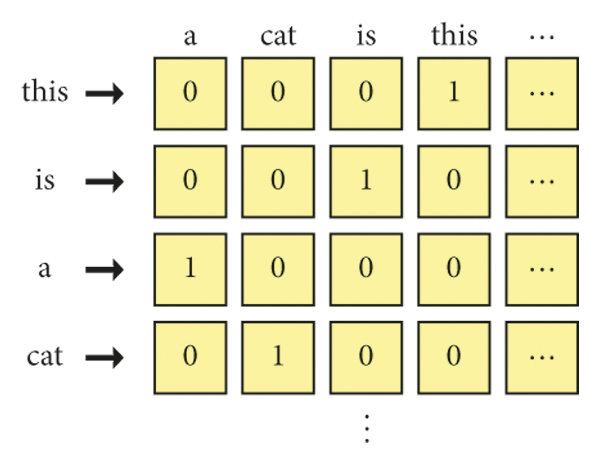
\includegraphics[scale=1.5]{assets/illustration_word_embedding.png}
      \caption{Ilustrasi \emph{Word Embedding}~\citep{Khan2021}}
      \label{fig:illustration_word_embedding}
\end{figure}

\emph{Word2Vec} merupakan salah satu bentuk implementasi dari \emph{Word Embedding} yang diajukan oleh
\citet{Mikolov2013} untuk mempelajari ekspresi dari sebuah kata termasuk juga arti
dan konteks dari kata tersebut~\citep{Jang2019}. \emph{Word2Vec} mampu memproses teks yang tidak
terstruktur dari korpus dan menghasilkan vektor sebagai keluaran dari korpus
tersebut~\citep{Nawangsari2019}. Setiap kata dari korpus dipetakan ke vektor yang berisi nilai
riil. Dengan mengubah kata menjadi vektor, kata yang memiliki makna yang sama akan direpresentasikan
berdekatan~\citep{Khattak2019}, kemiripan kata tersebut di hitung menggunakan \emph{cosine similarity}
dari vektor kata tersebut~\citep{Jang2019}. Arsitektur dari \emph{Word2Vec} ada dua yang pertama adalah \emph{Continous-Bag-Of-Words}
(CBOW) dan \emph{Skip-Gram}~\citep{Khattak2019}.

\begin{itemize}
      \item \emph{\bfseries Continous Bag Of Words} (CBOW)\\
      \emph{Continous Bag Of Words} adalah arsitektur dari \emph{Word2Vec} yang mana kata yang
      berada di sekitar kata target digunakan untuk memprediksi kata target tersebut. Prinsip
      dasar dari CBOW ini adalah memprediksi kata yang muncul berdasarkan kata
tetangga~\citep{Jang2019}. Arsitektur dari CBOW dapat diilustrasikan dengan Gambar~\ref{fig:cbow_Word2Vec}.

      \begin{figure}[H]
            \centering
            \includegraphics[scale=0.7]{assets/cbow_Word2Vec.jpg}
            \caption{Arsitektur \emph{CBOW}~\citep{Jang2019}}
            \label{fig:cbow_Word2Vec}
      \end{figure}

      \item \emph{\bfseries Continous Skip Gram}\\
      \emph{Continous Skip Gram} adalah arsitektur dari \emph{Word2Vec} merupakan kebalikan dari
      \emph{CBOW} yang mana satu kata digunakan untuk memprediksi kata sekitar. Prinsip dasar dari
      \emph{Skip-Gram} ini adalah memprediksi kata tetangga yang ada disekitar kata
      tersebut~\citep{Jang2019}. Arsitektur dari \emph{Skip-Gram} dapat diilustrasikan dengan
Gambar~\ref{fig:skip_gram_Word2Vec}.

      \begin{figure}[H]
            \centering
            \includegraphics[scale=0.7]{assets/skipgram_Word2Vec.jpg}
            \caption{Arsitektur \emph{Skip Gram}~\citep{Jang2019}}
            \label{fig:skip_gram_Word2Vec}
      \end{figure}
      
\end{itemize}

\subsection{\emph{Artificial Neural Network}}
\emph{Artificial Neural Network} (ANN) adalah pendekatan untuk memungkinkan mesin atau komputer
belajar yang terinspirasi dari cara manusia dan hewan belajar. ANN mempelajari sesuatu dengan cara
melakukan ribuan iterasi pembelajaran untuk memprediksi sesuatu berdasarkan hasil dari pembelajaran
tersebut. ANN terdiri dari beberapa lapisan simpul yang mirip dengan neuron pada otak manusia. Setiap
hasil dari lapisan simpul tersebut digunakan sebagai masukan untuk lapisan simpul selanjutnya~\citep{Desai2021}
seperti pada Gambar~\ref{fig:ann_illustration}.

ANN terdiri dari 3 lapisan \emph{(layer)}, lapisan yang pertama adalah lapisan masukan, lapisan kedua
adalah lapisan tersembunyi \emph{(hidden layer)}, dan yang ketiga adalah lapisan keluaran. Setiap lapisan
tersebut terdiri dari beberapa simpul \emph{(node)} yang terhubung ke simpul lainnya, setiap simpul
tersebut memiliki nilai ambang \emph{(Threshold)} dan nilai bobot \emph{(Weight)}.

Ketika lapisan masukan sudah ditentukan maka bobot akan mulai diinisialisasikan, kegunaan
dari bobot ini adalah untuk menentukan seberapa penting sebuah variabel dari masukan sebelumnya, dengan
nilai bobot yang besar akan mempengaruhi secara signifikan terhadap keluaran jika dibandingkan dengan
nilai masukan lainnya.


\begin{figure}[H]
      \centering
      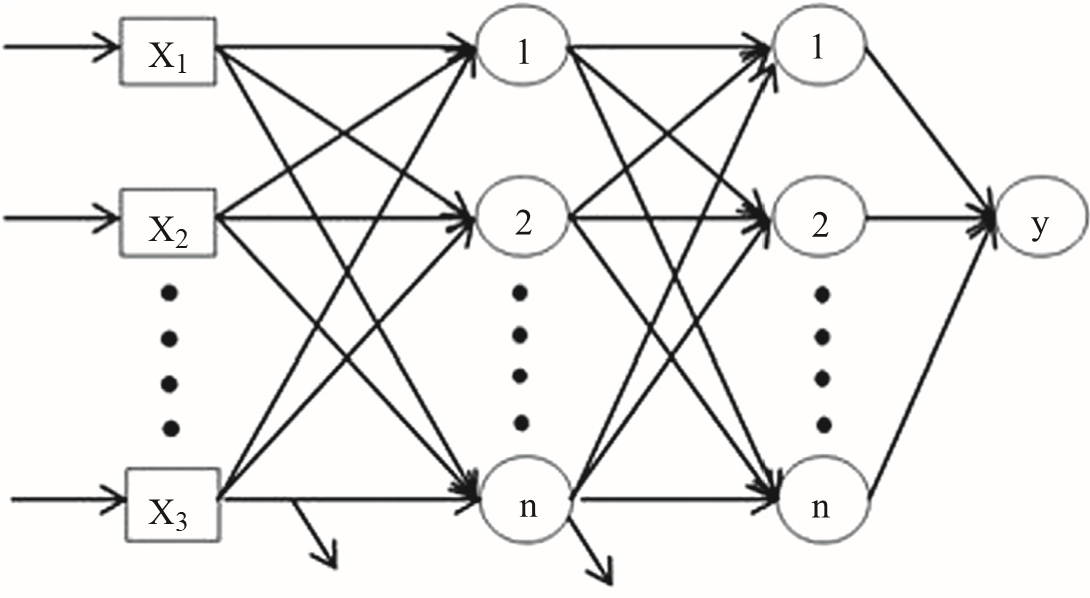
\includegraphics[scale=1]{assets/artificial_neural_network_structure.png}
      \caption{Ilustrasi ANN~\citep{Sairamya2019}}
      \label{fig:ann_illustration}
\end{figure}

\subsection{\emph{Convolutional Neural Network}}\label{CNN}
\emph{Convolutional Neural Network} (CNN) adalah \emph{feedforward neural network} yang umumnya
digunakan pada bidang \emph{computer vision}. Pendekatan CNN terinspirasi dari bagaimana cara kerja
otak manusia, dan hewan dalam mengenali gambar~\citep{Zhang2018}. Tidak seperti ANN yang lain CNN memiliki
kemampuan yang unik yaitu dapat menggabungkan ekstraksi fitur dan klasifikasi dalam satu pembelajaran
dan mengurangi keperluan untuk mengekstraksi fitur secara manual~\citep{Kiranyaz2019}. Karena hasil yang baik pada CNN
dalam pengenalan gambar, dan banyak digunakan sebagai metode klasifikasi dibarengi dengan suksesnya
klasifikasi \emph{ImageNet} dengan \emph{ConvNets} dengan landasan tersebut CNN juga dapat diaplikasikan pada
bidang analisis sentimen. Untuk menerapkan CNN pada bidang analisis sentimen maka diperlukan
penyesuaian data yang diberikan pada CNN agar dapat memahami data selain gambar dengan baik. Dalam
bidang pemrosesan bahasa alami penerapan CNN biasanya menggunakan teks yang sudah di vektorisasi sebagai
masukan yang akan diambil fiturnya dan fitur tersebut digunakan sebagai masukan pada lapisan \emph{convolution}.
Setiap simpul dari lapisan \emph{convolution} menyesuaikan dengan \emph{convolution kernel}
yang berfungsi menggabungkan masukan dari lapisan sebelumnya dengan beberapa bobot dan beberapa output
fitur untuk dijadikan masukan ke lapisan berikutnya~\citep{Wu2019}. CNN umumnya memiliki 3 lapisan
utama yaitu \emph{Convolution Layer}, \emph{Pooling Layer}, dan \emph{Fully Connected Layer}.

\begin{itemize}
      \item \emph{\bfseries Convolution Layer}\\ 
      \emph{Convolution Layer} adalah proses dimana masukan matriks dilakukan operasi konvolusi dengan
      filter yang memiliki ukuran lebih kecil dari masukan matriks untuk diekstraksi fiturnya.
      Dikarenakan ukuran filter lebih kecil dari masukan matriks setiap filter akan bergerak ke
      seluruh bagian dari masukan matriks dengan melakukan operasi konvolusi pada filter~\citep{Abdurrahman2020}.
      keluaran dari hasil operasi konvolusi akan diaplikasikan fungsi aktivasi \emph{non-linear} pada keluaran. Fungsi aktivasi
      yang digunakan pada \emph{Convolution Layer} adalah \emph{ReLU} dikarenakan
      \emph{ReLU} dapat mempercepat pembelajaran~\citep{Li2021}

      \item \emph{\bfseries Pooling Layer}\\
      \emph{Pooling Layer} atau dapat disebut juga dengan \emph{non-linear down-sampling} yang berfungsi
      untuk mereduksi dimensi dan mengurangi jumlah parameter dari hasil dari lapisan \emph{convolution}
      agar mengurangi biaya komputasi dan kalkulasi, dan untuk mengurangi \emph{overfitting} agar
      akurasi dari pengujian semakin dekat dengan akurasi latih~\citep{Wu2019}. Terdapat dua cara
      untuk melakukan \emph{pooling} yang pertama adalah \emph{Max Pooling} dan yang kedua adalah
      \emph{Average Pooling} tapi yang paling sering dipakai adalah \emph{Max Pooling} dikarenakan
      \emph{Max Pooling} dapat mempercepat konvergensi, mengambil fitur yang unggul, dan meningkatkan
      generalisasi~\citep{Chen2020}. Ilustrasi dari \emph{Max Pooling} dapat dilihat pada
      Gambar~\ref{fig:1d_max_pooling}

      \begin{figure}[H]
            \centering
            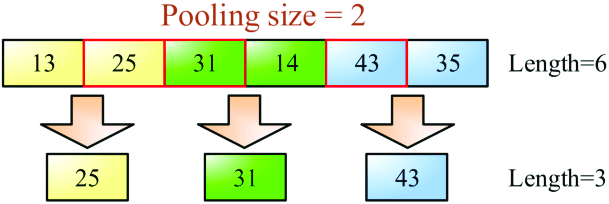
\includegraphics[scale=0.5]{assets/1d_max_pooling.png}
            \caption{Ilustrasi dari \emph{Max Pooling}~\citep{Kuo2018}}
            \label{fig:1d_max_pooling}
      \end{figure}

      \item \emph{\bfseries Fully Connected Layer}\\
      \emph{Fully Connected Layer} menerima vektor fitur sebagai masukan dan menggunakannya
      untuk mengklasifikasikan kalimat, dalam lapisan ini akan diaplikasikan regulasi untuk
      mengurangi \emph{overfitting}~\citep{Abdurrahman2020}. \emph{Fully Connected Layer} berfungsi
      untuk memastikan setiap \emph{neuron} dalam lapisan sebelumnya terkoneksi dengan \emph{neuron}
      pada lapisan berikutnya~\citep{Pandey2022}. Pada lapisan ini umumnya menggunakan aktivasi
      fungsi \emph{Softmax} untuk klasifikasi yang lebih dari dua label dan \emph{Sigmoid} untuk
      klasifikasi dua label~\citep{Li2021}.
\end{itemize}

\emph{Softmax} biasa disebut juga \emph{softargmax} berfungsi untuk mengubah sebuah vektor $K$ yang
bernilai rill menjadi vektor $K$ yang bernilai rill dalam bentuk distribusi probabilitas dari $K$
kemungkinan yang akan terjadi dan apa bila nilainya dijumlahkan akan bernilai 1~\citep{Wood2019}.

\begin{equation}\label{eq:softmax}
      \sigma(z_i) = \frac{e^{z_{i}}}{\sum_{j=1}^K e^{z_{j}}}
\end{equation}

Keterangan:
\begin{itemize}
      \item $z_i = vektor \ masukan$
      \item $K = jumlah \ kelas$
\end{itemize}

\emph{Rectified Linear Unit (ReLu)} adalah fungsi aktivasi yang umumnya digunakan pada jaringan
syaraf tiruan untuk mendapatkan nilai aktivasi yang sesuai pada setiap \emph{neuron}. Alasan penggunaan
\emph{ReLU} daripada fungsi aktivasi yang lain adalah \emph{ReLU} dapat mempercepat waktu latih dari
jaringan syaraf tiruan dikarenakan hasil turunan dari \emph{ReLU} adalah 1 untuk masukan yang
bernilai positif dan 0 untuk masukan yang negatif dengan kata lain \emph{neuron} hanya akan
diaktifkan ketika nilainya bernilai positif~\citep{Li2021}. Persamaan dari \emph{ReLU} dapat dilihat pada persamaan
\ref{eq:relu} dan \ref{eq:relu2} untuk grafik \emph{ReLU} dapat di lihat di Gambar~\ref{fig:relu}

\begin{figure}[H]
      \centering
      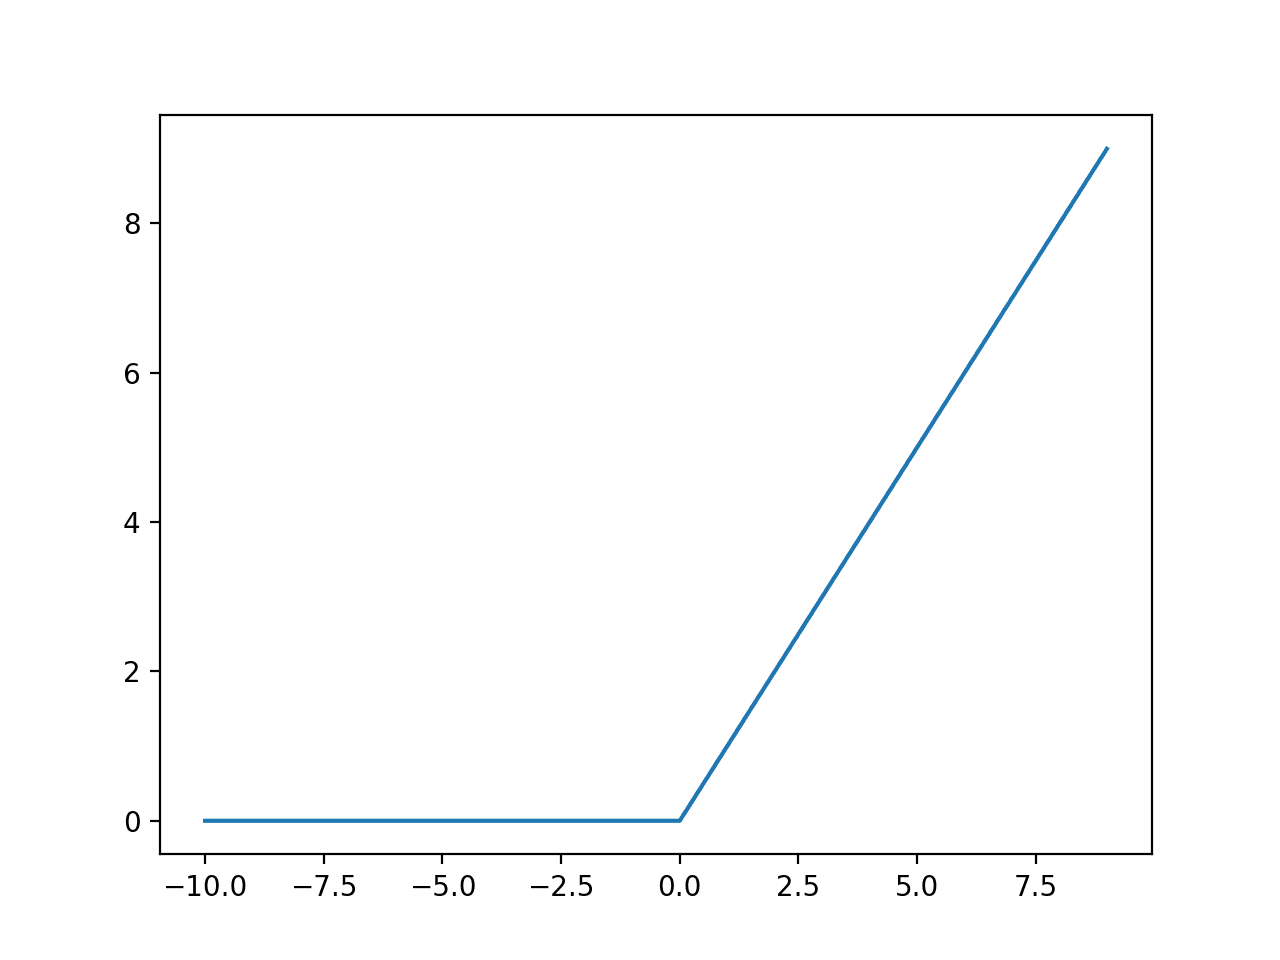
\includegraphics[scale=0.2]{assets/rectified_linear_unit.png}
      \caption{Contoh Grafik dari \emph{ReLU}}
      \label{fig:relu}
\end{figure}

\begin{equation}\label{eq:relu}
      ReLU(x) = \max(0, x)
\end{equation}


\begin{equation}\label{eq:relu2}
      ReLU(x) = \begin{cases}
            0, & \text{if } x < 1  \\
            x, & \text{if } x >= 0 \\
      \end{cases}
\end{equation}

Keterangan:
\begin{itemize}
      \item $x = nilai \ masukan$
\end{itemize}

CNN juga memiliki beberapa parameter yang disebut \emph{hyperparameter}, seperti berapa jumlah filter
(\emph{number of filter}), ukuran filter (\emph{filter size}), \emph{dropout} dan sebagainya.
Peningkatan performa pada CNN akan terjadi apabila nilai dari parameter tersebut
dioptimalkan~\citep{Akhter2020}.

\subsection{\emph{Confusion Matrix}}\label{Confusion Matrix}
\emph{Confusion Matrix} adalah cara untuk mengukur performa dari sistem klasifikasi berdasarkan
data yang dilatih dan data yang diuji. \emph{Confusion Matrix} berbentuk matriks dua dimensi,
dimensi pertama adalah label atau kelas yang asli, dan dimensi yang lain adalah label atau kelas
hasil dari sistem klasifikasi~\citep{Deng2016}. Ada 4 nilai yang dihasilkan dari \emph{Confusion Matrix},
diantaranya \emph{True Positive (TP)}, \emph{False Positive (FP)}, \emph{False Negative (FN)}, dan
\emph{True Negative (TN)} seperti pada Gambar~\ref{fig:ilustrasi_confusion_matrix}.

\begin{itemize}
      \item \emph{\bfseries True Positive (TP)} adalah nilai hasil prediksi positif dan nilai sebenarnya positif.
      \item \emph{\bfseries True Negative (TN)} adalah nilai hasil prediksi negatif dan nilai sebenarnya negatif.
      \item \emph{\bfseries False Positive (FP)} adalah nilai hasil prediksi positif dan nilai sebenarnya negatif.
      \item \emph{\bfseries False Negative (FN)} adalah nilai hasil prediksi negative dan nilai sebenarnya positif.
\end{itemize}

\begin{figure}[H]
      \centering
      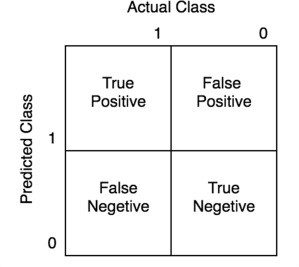
\includegraphics[scale=1]{assets/confusion_matrix.jpg}
      \caption{Ilustrasi \emph{Confusion Matrix}~\citep{Sharma2022}}
      \label{fig:ilustrasi_confusion_matrix}
\end{figure}


Hasil dari nilai \emph{confusion matrix} tadi dapat dijadikan beberapa metrik yaitu \emph{Precision},
\emph{Sensitivity (Recall)}, \emph{F-Measure (F1-Score)}, dan \emph{Accuracy}.


\begin{itemize}
      \item \emph{\bfseries Precision}\\
      \emph{Precision} adalah metrik yang digunakan untuk mengukur berapa banyak prediksi yang benar
      dalam total prediksi yang dilakukan. Cara penghitungan \emph{Precision} adalah prediksi yang
      benar dibagi total prediksi yang telah dilakukan. \emph{Precision} dapat dihitung menggunakan
      persamaan~\ref{eq:Precision}.

      \begin{equation}\label{eq:Precision}
            Precision = \frac{TP}{TP + FP}
      \end{equation}

      \item \emph{\bfseries \emph{Sensitivity (Recall)}}\\
      \emph{Sensitivity (Recall)} adalah metrik yang digunakan untuk mengukur berapa banyak prediksi yang
      benar dalam jumlah kelas atau label yang ada. Nilai tertinggi dalam \emph{Sensitivity (Recall)}
      adalah 1,0 dan nilai yang terendah adalah 0,0. \emph{Sensitivity (Recall)} dapat dihitung menggunakan
      persamaan~\ref{eq:Sensitivity_recall}.

      \begin{equation}\label{eq:Sensitivity_recall}
            Sensitivity = \frac{TP}{TP + FN}
      \end{equation}

      \item \emph{\bfseries F-Measure (F1-score)}\\
      \emph{F-Measure (F1-Score)} adalah rata-rata harmonik dari \emph{Precision} dan \emph{Sensitivity (Recall)}, berguna
      untuk menyeimbangkan nilai dari \emph{Precision} dan \emph{Sensitivity (Recall)} nilai \emph{F-Measure (F1-Score)} akan
      tinggi jika nilai dari \emph{Precision} dan \emph{Sensitivity (Recall)} tinggi dan akan rendah jika nilai dari
      \emph{Precision} dan \emph{Sensitivity (Recall)} rendah. \emph{F-Measure (F1-Score)} dapat dihitung menggunakan
      persamaan~\ref{eq:f_score_f_measure}.

      \begin{equation}\label{eq:f_score_f_measure}
            F-Measure = 2 \times \frac{Recall \times Precision}{Recall + Precision}
      \end{equation}

      \item \emph{\bfseries Accuracy}\\
      \emph{Accuracy} atau akurasi merupakan salah satu metrik yang biasa digunakan untuk mengevaluasi
      kinerja model pada semua kelas atau label. Metrik ini berguna ketika kelas memiliki bobot yang
      setara dengan kelas yang lainnya. Cara penghitungan metrik adalah rasio antara jumlah prediksi
      yang benar dengan jumlah total prediksi. \emph{Accuracy} dapat dihitung menggunakan
      persamaan~\ref{eq:Accuracy}.

      \begin{equation}\label{eq:Accuracy}
            Accuracy = \frac{(TP + TN)}{(TP + FP + TN + FN)}
      \end{equation}

\end{itemize}

\subsection{\emph{Rational Unified Process} (RUP)}
\emph{Rational Unified Process} (RUP) adalah salah satu metode pengembangan perangkat lunak yang
menerapkan konsep orientasi objek dan umumnya digunakan untuk pengembangan aplikasi
berbasis \emph{web}. Tujuan dari RUP adalah untuk memastikan perangkat lunak yang dikembangkan
berkualitas tinggi yang memenuhi ekspektasi dari pengguna. Dalam skala besar RUP bersifat bersambung,
namun dalam skala kecil RUP bersifat iteratif dan bertahap untuk perilisan
\emph{software}-nya~\citep{anwar2014review}. RUP ditemukan dan dikembangkan oleh
Rational\textregistered~Software. RUP terdiri dari empat fase bersifat iteratif yaitu Fase Insepsi,
Fase Elaborasi, Fase Konstruksi dan Fase Transisi seluruh fase tersebut dapat diilustrasikan pada Gambar~\ref{fig:rup}.

\begin{itemize}
      \item \emph{\bfseries Fase Insepsi}\\ 
      Fase Insepsi terdiri dari mendifinisikan kasus bisnis,
      membatasi ruang lingkup proyek, menentukan kebutuhan dari perangkat lunak dan mendesain perangkat
      lunak sesuai dengan kasus bisnis.

      \item \emph{\bfseries Fase Elaborasi}\\
      Fase Elaborasi adalah menganalisa berbagai persyaratan dan resiko dalam pengembangan perangkat
      lunak. Elaborasi juga memastikan arsitektur, kebutuhan, dan perencanaan stabil dan tidak banyak
      yang diubah ketika ada perubahan.

      \item \emph{\bfseries Fase Konstruksi}\\
      Fase Konstruksi adalah fase dimana perangkat lunak mulai
      diimplementasikan dalam bentuk kode program sesuai dengan kebutuhan bisnis dan kebutuhan dari
      perangkat lunak tersebut. Setiap kode program yang sudah diimplementasikan akan diuji.

      \item \emph{\bfseries Fase Transisi}\\
      Fase Transisi adalah fase perangkat lunak mulai disebarkan pada pengguna, apabila perangkat
      lunak masih memiliki masalah atau terdapat ketidaksesuaian dengan yang diekspektasikan oleh
      pengguna maka program akan dikembangkan lagi dan dirilis ulang dengan penundaan pada penambahan
      fitur atau perbaikan masalah.

\end{itemize}

\begin{figure}[H]
      \centering
      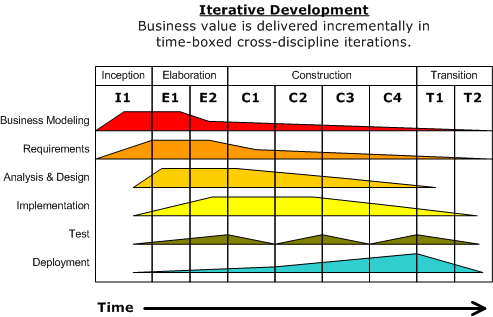
\includegraphics[scale=0.7]{assets/rup.png}
      \caption{Fase RUP}
      \label{fig:rup}
\end{figure}

\section{Pustaka (\emph{Library \& Framework}) yang Digunakan}

\begin{itemize}
      {\bfseries \item \emph{Tensorflow}}\\
      Dilansir dari website resminya \emph{Tensorflow} adalah \emph{platform} ujung-ke-ujung (\emph{end-to-end})
      dengan sumber terbuka (\emph{open source}) untuk membuat model pembelajaran
      mesin (\emph{machine learning}). \emph{Tensorflow} mempermudah pemula dan ahli untuk membuat model
      pembelajaran mesin (\emph{machine learning})~\citep{tensorflow2015-whitepaper}. Ada 2 cara yang
      dapat dilakukan untuk menyebarkan model machine learning pada aplikasi \emph{mobile} menggunakan
      \emph{Tensorflow} yaitu \emph{Tensorflow Lite} dan \emph{Tensorflow Serving}.

      \begin{itemize}
            {\bfseries \item \emph{Tensorflow Lite}} Dilansir dari website resminya \emph{Tensorflow Lite}
            adalah pustaka (\emph{library}) untuk menyebarkan (\emph{deploy}) model \emph{machine learning} pada \emph{mobile}
            (\emph{handphone}), \emph{microcontroller}, dan peranti yang memiliki sumber daya yang
            sedikit~\citep{tensorflow2015-whitepaper}.

            {\bfseries \item \emph{Tensorflow Serving}} Dilansir dari website resminya \emph{Tensorflow Serving}
            adalah cara yang fleksibel, berperforma tinggi untuk menyebarkan model \emph{machine learning}
            pada \emph{server}~\citep{tensorflow2015-whitepaper}.
      \end{itemize}

      {\bfseries \item \emph{Scikit-Learn}}\\
      Dilansir dari website resminya \emph{Scikit-Learn} adalah pustaka (\emph{Library}) untuk bahasa pemrograman
      python yang menyediakan banyak alat untuk melakukan pembelajaran mesin (\emph{machine-learning}) secara
      diawasi (\emph{supervised}) dan tidak diawasi (\emph{unsupervised})~\citep{scikit-learn}. Fitur-fitur
      yang ada di \emph{scikit-learn} yaitu klasifikasi, regresi, klusterisasi, reduksi dimensi,
      pemilihan model, dan praproses.

      {\bfseries \item \emph{Gensim}}\\
      Dilansir dari website resminya \emph{Gensim} atau \emph{Generate Similar} adalah pustaka untuk bahasa
      pemrograman python yang berfungsi untuk merepresentasikan dokumen sebagai vektor semantik seefisien mungkin dan semudah
      mungkin. \emph{Gensim} didesain untuk memproses data yang tidak terstruktur atau \emph{(`Plain Text')}
      menggunakan algoritma pembelajaran mesin yang tidak diawasi~\citep{rehurek_lrec}. Algoritma yang
      tersedia pada Gensim adalah \emph{Word2Vec}, \emph{FastText} dan sebagainya.

      {\bfseries \item \emph{Google-Play-Scraper}}\\
      Dilansri dari website github dan pypi \emph{Google-Play-Scraper} adalah pustaka untuk bahasa pemrograman
      python yang berfungsi untuk memudahkan \emph{web crawling} pada website \emph{Google Play Review}.

      {\bfseries \item Sastrawi}\\
      Dilasir dari website github dan pypi Sastrawi adalah pustaka untuk bahasa pemrograman python yang
      berfungsi untuk melakukan \emph{stemming} dan menghilangkan \emph{stopword} pada bahasa indonesia.

\end{itemize}

\section{Penelitian Yang Relevan}
\citet{Sharma2020} menggunakan CNN dan \emph{pre-trained Word2Vec} untuk analisis sentimen pada
dataset IMDb \emph{movie review} berjumlah 5331 berlabel positif dan 5331 berlabel negatif dan di
praproses dengan cara mengubah \emph{multilingual} data menjadi Bahasa Inggris, \emph{Tokenize} pada
setiap spasi, menghapus pungtuasi, menghapus stoword, menghapus kata dengan panjang \leq~1 karakter,
dan teks diubah menjadi \emph{lowercase} menghasilkan model dengan akurasi sebesar 99,07\% pada data
latih dan 82,19\% pada data uji. Dari penelitian ini dapat disimpulkan bahwa CNN dan \emph{Word2Vec}
sangat efektif dan efisien untuk analisis sentimen.

\citet{Dong2020} menggunakan CNN untuk analisis sentimen perkalimat pada dataset saham yang sudah
di praproses dengan cara menghilangkan angka dan karakter spesial, \emph{stemming}, \emph{casefolding},
dan \emph{tokenize}. Menghasilkan model dengan akurasi 98,1\% dibandingkan dengan \emph{SVM (Support Vector Machine)} yang
memiliki akurasi 90\% dan \emph{Random Forest} memiliki akurasi 93\%. Dari hasil penelitian tersebut
dapat diambil kesimpulan bahwa CNN melebihi akurasi dari \emph{SVM (Support Vector Machine)} dan
\emph{Random Forest}.

\citet{Smetanin2019} menggunakan CNN dan \emph{pre-trained Word2Vec} yang dilatih dari 5.5 juta \emph{review}
untuk analisis sentimen pada produk \emph{review} dalam bahasa Rusia dari kategori `Women's Clothes and Accessories'
berjumlah 821 ribu \emph{review} yang dilabel secara otomatis dan di praproses dengan cara \emph{lowercase},
mengubah emotikon menjadi \emph{emotional tag}, dan normalisasi teks. Mendapatkan hasil dengan
\emph{Precision} 75,63\%, \emph{Recall} 75,31\% dan \emph{F1-score} 75,45\% yang kemudian dibandingkan
dengan algoritma pembelajaran mesin \emph{Multinomial Naive Bayes} dengan hasil \emph{Precision} 74,47\%,
\emph{Recall} 73,79\% dan \emph{F1-score} 73,90\%. Dari penelitian ini dapat diambil kesimpulan
bahwa CNN dan \emph{Word2Vec} dapat melebihi kinerja dari \emph{Multinomial Naive Bayes}.

\citet{Amanatidis2019} menggunakan CNN dan \emph{Word2Vec} yang sudah dilatih terlebih dahulu dengan
menggunakan dataset IMDb \emph{movie review} untuk melakukan analisis sentimen pada data \emph{review}
TripAdvisor, setiap \emph{review} dipraproses dengan cara \emph{lowercase}, menghapus pungtuasi,
mempadding \emph{review}, dan memotong \emph{review} yang lebih dari 1000 kata. Hasil dari CNN yang di
latih dengan menggunakan dataset IMDb \emph{movie review} menghasilkan akurasi 88,85\%. Dari hasil penelitian
tersebut dapat disimpulkan bahwa CNN dan \emph{Word2Vec} dapat dengan mudah menghasilkan akurasi 88,85\%.

\citet{Aldiansyah2019} menggunakan CNN dan \emph{Word2Vec} untuk analisis sentimen pada opini publik
untuk jaringan 4G Smartfren yang berjumlah 1120 kicauan yang dilabeli secara manual menjadi dua label
yang berjumlah 560 positif dan 560 negatif. Kicauan tersebut dipraproses dengan cara \emph{casefolding},
\emph{tokenization}, penghapusan pungtuasi, pengahapusan \emph{stopword}, dan \emph{stemming} menghasilkan
model dengan akurasi 88,21\%.

\section{Kesimpulan}
Bab ini sudah memberikan landasan teori dari beberapa literatur dan juga memberikan penjelasan dari
penelitian lain yang relevan dengan penelitian yang dilakukan yaitu analisis sentimen menggunakan CNN\@.